% !TeX root = surprises.tex

\chapter{¿Son congruentes los triángulos con áreas y perímetros iguales?}\label{c.congruent}

%%%%%%%%%%%%%%%%%%%%%%%%%%%%%%%%%%%%%%%%%%%%%%%%%%%%%%%%%%%%%%%

¿Son congruentes dos triángulos con la misma área y el mismo perímetro? No necesariamente: los triángulos con lados $(17,25,28)$ y $(20,21,29)$ tienen ambos perímetro $70$ y área $210$ pero no son congruentes (Fig.~\ref{f.congruent-first-example})\footnote{Las áreas se calcularon mediante la fórmula de Herón (Teorema~\ref{thm.heron}) y los ángulos mediante la ley de los cosenos (Teorema~\ref{thm.law-of-cosines}).}. Este capítulo muestra que dado un triángulo de lados racionales es posible construir un triángulo no congruente, también de lados racionales, que tenga la misma área y el mismo perímetro.
Llevamos a cabo la derivación utilizando un ejemplo, mostrando que el triángulo de lados $(3,4,5)$ y el triángulo de lados 
$\left(\frac{156}{35}, \frac{101}{21}, \frac{41}{15}\right)$ tienen ambos perímetro $12$ y área $6$.

\begin{figure}[b]
\begin{center}
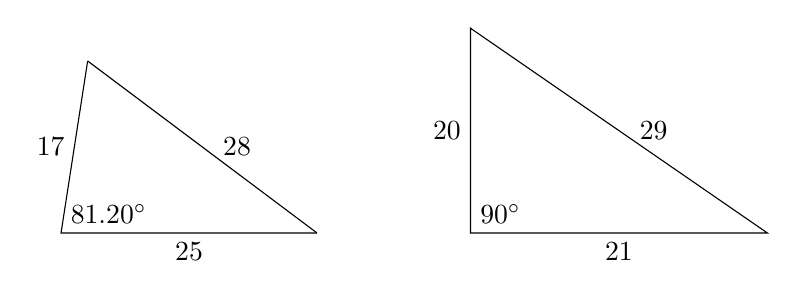
\begin{tikzpicture}[scale=1.3]
\coordinate (A1) at (0,0);
\node[above right] at (A1) {$81.20^\circ$};
\coordinate (B1) at (2.5cm,0);
\coordinate (C1) at (81.20:1.7cm);
\draw (B1) -- node[below] {$25$} (A1) -- node[left] {$17$} (C1);
\draw (B1) -- node[right,xshift=4pt] {$28$} +(143.13:2.8cm);
\begin{scope}[xshift=4cm]
\coordinate (A2) at (0,0);
\node[above right] at (A2) {$90^\circ$};
\coordinate (B2) at (2.9cm,0);
\coordinate (C2) at (0,2cm);
\draw (B2) -- node[below] {$21$} (A2) -- node[left] {$20$} (C2) -- node[right,xshift=4pt] {$29$} cycle;
\end{scope}
\end{tikzpicture}
\end{center}
\caption{Triángulos no congruentes con la misma área y el mismo perímetro}\label{f.congruent-first-example}
\end{figure}

\section{De un triángulo a una curva elíptica}\label{s.elliptic}

Las tres bisectrices de los ángulos de un triángulo se intersecan en un punto llamado \emph{éncentro} del triángulo. El incentro es el centro de una circunferencia inscrita en el triángulo (Fig.~\ref{f.congruent1}). 

Deja caer altitudes desde el centro $O$ a los lados. Las altitudes tienen longitud $r$, el radio de la circunferencia inscrita. Las altitudes y las bisectrices de los ángulos crean tres pares de triángulos rectángulos congruentes:
\[
\triangle AOB'\cong \triangle AOC',\quad \triangle BOA'\cong \triangle BOC',\quad \triangle COA'\cong \triangle COB'\,.
\]

\begin{figure}[t]
\begin{center}
\begin{tikzpicture}[scale=1.85]
% Draw base and path two lines at known angles
\draw (0,0) coordinate (a) node[below] {$A$} --
  (0:6) coordinate (b) node[below] {$B$};
\path[name path=ac] (a) -- +(50:4);
\path[name path=bc] (b) -- +(150:5);
% Get their intersection and draw lines between vertices
\path[name intersections={of=ac and bc,by=c}];
\node[above] at (c) {$C$};
\draw (a) -- (c) -- (b) -- (a);
% Label angles with tick marks
\draw (a) ++(0:4mm) arc (0:50:4mm);
\draw (a) ++(10:3.5mm) -- +(10:1mm);
\draw (a) ++(15:3.5mm) -- +(15:1mm);
\draw (a) ++(35:3.5mm) -- +(35:1mm);
\draw (a) ++(40:3.5mm) -- +(45:1mm);
\draw (b) ++(150:5mm) arc (150:180:5mm);
\draw (b) ++(157.5:4.5mm) -- +(157.5:1mm);
\draw (b) ++(172.5:4.5mm) -- +(172.5:1mm);
\draw (c) ++(230:3mm) arc (230:330:3mm);
\draw (c) ++(250:2.5mm) -- +(250:1mm);
\draw (c) ++(255:2.5mm) -- +(255:1mm);
\draw (c) ++(260:2.5mm) -- +(260:1mm);
\draw (c) ++(300:2.5mm) -- +(300:1mm);
\draw (c) ++(305:2.5mm) -- +(305:1mm);
\draw (c) ++(310:2.5mm) -- +(310:1mm);
% Path bisectors of two lines
\path[name path=bia] (a) -- +(25:3.5);
\path[name path=bib] (b) -- +(165:5);
% Intersection of angle bisectors
\path [name intersections={of=bia and bib,by=center}];
% Draw angle bisectors to center
\draw (a) -- (center);
\draw (c) -- (center);
\draw (b) -- (center);
% Draw radii
\draw (center) -- node[left] {$r$}
  ($(a)!(center)!(b)$) node[below,yshift=-2pt] {$C'$}
  coordinate (ap);
\draw (center) -- node[left,yshift=-4pt] {$r$}
  ($(a)!(center)!(c)$) node[above left,xshift=4pt] {$B'$}
  coordinate (bp);
\draw (center) -- node[right] {$r$}
  ($(b)!(center)!(c)$) node[above right] {$A'$}
  coordinate (cp);
\vertex{center};
\node[above,xshift=3pt,yshift=6pt] at (center) {$O$};
% Draw right angle squares
\draw (ap) rectangle +(3pt,3pt);
\draw[rotate=-40] (bp) rectangle +(3pt,3pt);
\draw[rotate=-120] (cp) rectangle +(3pt,3pt);
% Labels of angles
\node[above,xshift=5pt,yshift=21pt]
  at (center) {$\gamma/2$};
\node[above left,xshift=-4pt,yshift=21pt]
  at (center) {$\gamma/2$};
\node[above right,xshift=4pt,yshift=-5pt]
  at (center) {$\beta/2$};
\node[below right,yshift=-6pt]
  at (center) {$\beta/2$};
\node[left,xshift=-8pt,yshift=3pt]
  at (center) {$\alpha/2$};
\node[below left,xshift=2pt,yshift=-6pt]
  at (center) {$\alpha/2$};
% Labels of line segments (names of points are weird...)
\path (a) -- node[below,yshift=-2pt] {$u$} (ap);
\path (a) -- node[left, xshift=-2pt] {$u$} (bp);
\path (b) -- node[above,yshift=2pt]  {$v$} (cp);
\path (b) -- node[below,xshift=-2pt] {$v$} (ap);
\path (c) -- node[above,xshift=-2pt] {$w$} (bp);
\path (c) -- node[above,xshift=2pt]  {$w$} (cp);
% Labels of sides
\draw[<->] ($(a)+(0,-10pt)$) -- node[fill=white] {$c$} 
           ($(b)+(0,-10pt)$);
\draw[<->] ($(a)+(-4pt,7pt)$) -- node[fill=white] {$b$}
           ($(c)+(-4pt,7pt)$);
\draw[<->] ($(b)+(2pt,9pt)$) -- node[fill=white] {$a$}
           ($(c)+(2pt,9pt)$);
% Inscribed circle
\node[draw,circle through=(ap)] at (center) {};
\end{tikzpicture}
\end{center}
\caption{Un círculo inscrito en un triángulo}\label{f.congruent1}
\end{figure}

Las altitudes dividen los lados $a,b,c$ en segmentos $u,v,w$. El área del $\triangle ABC$ es la suma de las áreas del $\triangle BOC, \triangle AOB, \triangle AOC$:
\begin{subeqnarray}
A &=& \frac{1}{2}(w+v)r + \frac{1}{2}(v+u)r + \frac{1}{2}(u+w)r\\
&=&\frac{1}{2}\cdot 2(u+v+w)r\\
&=&\frac{1}{2}(a+b+c)r\\
&=&sr\,, \slabel{eq.area1}
\end{subeqnarray}
donde $s$ es el \emph{semiperímetro}, la mitad del perímetro del triángulo $\triangle ABC$. Las longitudes de $u,v,w$ se pueden expresar utilizando el radio de la circunferencia y los ángulos centrales $\alpha/2,\beta/2,\gamma/2$:
\begin{align}
\tan \frac{\alpha}{2}= \frac{u}{r},\quad
\tan \frac{\beta}{2} = \frac{v}{r},\quad
\tan \frac{\gamma}{2} =\frac{w}{r}\,.\label{eq.uvw}
\end{align}
El semiperímetro puede expresarse ahora en términos de las tangentes:
\[
s = u+v+w = r\tan \frac{\alpha}{2}+r\tan \frac{\beta}{2}+r\tan \frac{\gamma}{2} = r\left(\tan \frac{\alpha}{2}+\tan \frac{\beta}{2}+\tan \frac{\gamma}{2}\right)\,,
\]
y por Eq.~\ref{eq.area1} el área es:
\begin{align}
A = sr = r^2\left(\tan \frac{\alpha}{2}+\tan \frac{\beta}{2}+\tan \frac{\gamma}{2}\right)\,.\label{eq.area2}
\end{align}
A partir de $r=A/s$, la Ecuación~\ref{eq.area2} puede escribirse como:
\begin{align}
\tan \frac{\alpha}{2}+\tan \frac{\beta}{2}+\tan \frac{\gamma}{2} = \frac{A}{r^2} = \frac{A}{(A/s)^2} = \frac{s^2}{A}\,.\label{eq.area3}
\end{align}
Ya que la suma de los ángulos $\alpha,\beta,\gamma$ es $360^\circ$:
\begin{subeqnarray}
\gamma/2 &=& 360^\circ/2 - (\alpha/2 + \beta/2)\\
\tan\gamma/2 &=& \tan(180^\circ - (\alpha/2 + \beta/2))\\
 &=& -\tan (\alpha/2 + \beta/2)\\
&=& \frac{\tan\alpha/2 + \tan\beta/2}{\tan\alpha/2 \, \tan\beta/2-1}\,,\slabel{eq.tangent1}
\end{subeqnarray}
utilizando la fórmula de la tangente de la suma de dos ángulos (Teorema~\ref{thm.tangent-sum}).

Simplifiquemos la notación definiendo variables para las tangentes:
\begin{align}
x=\tan \frac{\alpha}{2},\quad
y=\tan \frac{\beta}{2},\quad
z=\tan \frac{\gamma}{2}\,.\label{eq.variables-for-tangents}
\end{align}
Por la Ecuación~\ref{eq.tangent1} podemos expresar $z=\tan\gamma/2$ en términos de $x,y$:
\begin{align}
z = \frac{x+y}{xy-1}\,.\label{eq.xy1}
\end{align}
Con esta notación, la Ecuación~\ref{eq.area3} se convierte en:
\begin{align}
x+y+\frac{x+y}{xy-1}=\frac{s^2}{A}\,.\label{eq.xy2}
\end{align}
Dados valores fijos de $A$ y $s$ ¿existen múltiples soluciones de Eq.~\ref{eq.xy2}?

Para el triángulo rectángulo $(3,4,5)$:
\begin{align}
\frac{s^2}{A} = \frac{\left(\frac{1}{2}(3+4+5)\right)^2}{\frac{1}{2}\cdot 3\cdot 4} = \frac{6^2}{6}=6\,.
\end{align}

\noindent{}Si hay otra solución Ecuación~\ref{eq.xy2} con $s^2/A=6$, se puede escribir como:
\begin{subeqnarray}
x+y+\frac{x+y}{xy-1}&=&6\\
x^2y + xy^2 -6xy + 6 &=& 0\,.\slabel{eq.elliptic}
\end{subeqnarray}
Esta es una ecuación para una \emph{curva elíptica}.

\section{Resolución de la ecuación de la curva elíptica}

Una porción de la gráfica de la Ecuación~\ref{eq.elliptic} se muestra Fig.~\ref{f.two-secants}. Cualquier punto de la curva cerrada en el primer cuadrante es una solución de la ecuación porque las longitudes de los lados del triángulo deben ser positivas. $A,B,D$ corresponden al triángulo $(3,4,5)$ como se muestra a continuación. Para encontrar soluciones racionales adicionales se utiliza el método de las dos secantes.

Construimos una secante a través de los puntos $ A = (2,3), B = (1,2) $. Corta la curva en $C=(-1,5,-0,5)$, pero no da solución porque los valores son negativos. Construimos una segunda secante desde $C$ hasta $D=(3,2)$. La intersección con la curva en $E\approx (1,5,1,2)$ da una nueva solución cuyas coordenadas se calcularán a continuación.

\begin{figure}[b]
\begin{center}
\begin{tikzpicture}[scale=1]
\draw[very thin,step=10mm] (-4,-4) grid (4,4);
\draw[thick] (-4,0) -- (4,0);
\draw[thick] (0,-4) -- (0,4);
\foreach \x in {-3,...,4}
  \node at (\x-.2,-.2) {\sm{\x}};
\foreach \y in {-3,...,-1}
  \node at (+.2,\y-.3) {\sm{\y}};
\foreach \y in {1,...,4}
  \node at (+.2,\y-.3) {\sm{\y}};

\draw[very thick,domain=.936:3.306,samples=200] plot (\x,{
(
  (6*\x-\x*\x)+
  sqrt(
   (\x*\x-6*\x)^2 -
   4*\x*6
  )
)/
(2*\x)
});

\draw[very thick,domain=.936:3.306,samples=100] plot (\x,{
(
  (6*\x-\x*\x)-
  sqrt(
   (\x*\x-6*\x)^2 -
   4*\x*6
  )
)/
(2*\x)
});

\draw[very thick,domain=-2.5:-.25,samples=100] plot (\x,{
(
  (6*\x-\x*\x)+
  sqrt(
   (\x*\x-6*\x)^2 -
   4*\x*6
  )
)/
(2*\x)
});

\coordinate (A) at (2,3);
\coordinate (B) at (1,2);
\coordinate (C) at (-1.5,-0.5);
\coordinate (D) at (3,2);
\coordinate (E) at (1.5,1.2);

\draw[very thick,dashed,red]  ($(C)!-.4!(A)$) -- ($(C)!1.2!(A)$);
\draw[very thick,dashed,blue] ($(C)!-.4!(D)$) -- ($(C)!1.2!(D)$);

\node[right,xshift=9pt,yshift=-5pt]  at (A)  {$A=(2,3)$};
\node[above left,xshift=-4pt]        at (B)  {$B=(1,2)$};
\node[right,xshift=23pt,yshift=-4]   at (C)  {$C=(-1.5,-0.5)$};
\node[right,xshift=8pt,yshift=-6pt]  at (D)  {$D=(3,2)$};
\node[below,xshift=15pt,yshift=-12pt] at (E) {$E=(1.5,1.2)$};
\vertexcolor{A}{red};
\vertexcolor{B}{red};
\vertexcolor{C}{purple};
\vertexcolor{D}{blue};
\vertexcolor{E}{blue!50!red};
\end{tikzpicture}
\end{center}
\caption{El método de las dos secantes}\label{f.two-secants}
\end{figure}

La ecuación de la recta (roja) que pasa por $A,B$ es $y=x+1$. En Eq.~\ref{eq.elliptic}:
\begin{eqnarray*}
x^2(x+1) + x(x+1)^2 -6x(x+1) +6 &=&0\\
2x^3 -3x^2 -5x +6 &=&0\,.
\end{eqnarray*}
De $A,B$ conocemos dos raíces $x=2,x=1$ por lo que podemos factorizar el polinomio cúbico:
\[
(x-2)(x-1)(ax+b)=0\,,
\]
donde la tercera raíz es desconocida. Multiplicamos los factores y concluimos que $a=2, b=3$ ya que $2x^3 -3x^2 -5x +6 = ax^3+\cdots+2b$. El tercer factor es $2x+3$ lo que da la tercera raíz $x=-\frac{3}{2}$ e $y=x+1=-\frac{1}{2}$. Este es el punto $C=(-\frac{3}{2},-\frac{1}{2})$ de la gráfica.

La ecuación de la recta (azul) que pasa por $C,D$ es:
\begin{align}
y = \frac{5}{9}x + \frac{1}{3}\,.\label{eq.second-secant}
\end{align}
Sustituir por $y$ en la Ecuación~\ref{eq.elliptic}:
\begin{eqnarray*}
x^2\left(\frac{5}{9}x + \frac{1}{3}\right) + x\left(\frac{5}{9}x + \frac{1}{3}\right)^2 -6x\left(\frac{5}{9}x + \frac{1}{3}\right) +6 &=&0\\
\frac{70}{81}x^3 - \frac{71}{27}x^2 - \frac{17}{9}x +6 &=&0\,.
\end{eqnarray*}
De $C,D$ sabemos dos raíces $x=3,x=-\frac{3}{2}$ por lo que podemos factorizar el polinomio cúbico:
\[
(x-3)\left(x+\frac{3}{2}\right)(ax+b)=0\,.
\]
Igualando los coeficientes del término cúbico y los términos constantes se obtiene:
\begin{eqnarray*}
\frac{70}{81}x - \frac{4}{3}&=&0\\
x&=& \frac{54}{35}\approx 1.543\,,
\end{eqnarray*}
y $y$ se puede calcular a partir de la Ecuación~\ref{eq.second-secant}:
\[
y=\frac{25}{21}\approx 1.190\,.
\]
Las coordenadas de $E$ son:
\[
\left(\frac{54}{35}, \frac{25}{21}\right)=(1.543,1.190)\,,
\]
que se acercan a las aproximaciones $(1,5,1,2)$ obtenidas del gráfico.

Por último, calcula $z$ a partir de la Ecuación~\ref{eq.xy1}:
\[
z=\frac{x+y}{xy-1}=%
\displaystyle\left(\frac{54}{35} + \frac{25}{21}\right)%
 \, \bigg/ \,%
\displaystyle\left(\frac{54}{35}\frac{25}{21}-1\right)=%
\frac{2009}{615} = \frac{49}{15}\,.
\]

\section{Derivación de un triángulo a partir de la curva elíptica}

Usando las Ecs.~\ref{eq.uvw}, \ref{eq.variables-for-tangents}, $a,b,c$, los lados del triángulo $\triangle ABC$, se pueden calcular a partir de $x,y,z$ y $r=A/s=6/6=1$:
\begin{eqnarray*}
a&=&w+v = r(z+y)=(z+y)\\
b&=&u+w= r(x+z)=(x+z)\\
c&=&u+v=r(x+y)=(x+y)\,.
\end{eqnarray*}
Para la solución $A$ de la curva elíptica los lados del triángulo son:
\begin{eqnarray*}
a &=& z+y = 1+3 = 4\\
b &=& x+z = 2+1=3\\
c &=& x+y = 2+3=5\,.
\end{eqnarray*}
Para la solución $E$ de la curva elíptica los lados del triángulo son:
\begin{eqnarray*}
a &=& z+y = \frac{49}{15} + \frac{25}{21} = \frac{156}{35}\\
&&\\
b &=& x+z = \frac{54}{35} + \frac{49}{15} = \frac{101}{21}\\
&&\\
c &=& x+y = \frac{54}{35} + \frac{25}{21} =\frac{41}{15}\,.
\end{eqnarray*}
Comprobemos este resultado. El semiperímetro es:
\[
s=\frac{1}{2}\left(\frac{156}{35} + \frac{101}{21}+\frac{41}{15}\right) = \frac{1}{2}\left(\frac{468+505+287}{105}\right) = \frac{1}{2}\left(\frac{1260}{105}\right)= 6\,,
\]
y el área puede calcularse mediante la fórmula de Heron (Teorema~\ref{thm.heron}):
\[
A= \sqrt{6 \left(6-\frac{156}{35}\right) \left(6-\frac{101}{21}\right) \left(6-\frac{41}{15}\right)}=\sqrt{36} = 6\,.
\]
¿Es $\left(\frac{156}{35}, \frac{101}{21}, \frac{41}{15}\right)\cong(3,4,5)$? Para simplificar el cálculo vamos a utilizar las aproximaciones decimales $(4,48,4,81,2,73)$. Entonces:
\[
\sqrt{4.48^2+2.73^2}=5.25\neq 4.81\,,
\]
por lo que no es un triángulo rectángulo y no es congruente con $(3,4,5)$.

La ley de los cosenos se puede utilizar para calcular los ángulos del triángulo como se muestra en Fig.~\ref{f.not-a-right-triangle}.


\begin{figure}[t]
\begin{center}
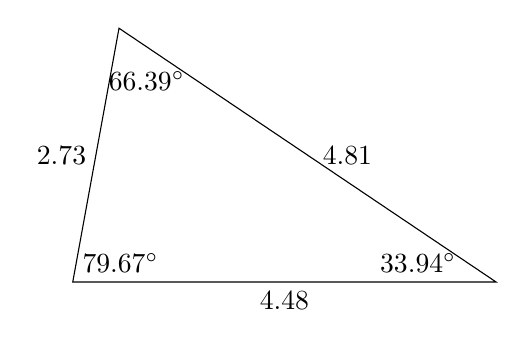
\begin{tikzpicture}[scale=1.2]
\coordinate (A1) at (0,0);
\coordinate (B1) at (4.48cm,0);
\coordinate (C1) at (79.67:2.73cm);
\node[above right] at (A1) {$79.67^\circ$};
\node[above left,xshift=-11pt] at (B1) {$33.94^\circ$};
\node[below,yshift=-12pt,xshift=10pt] at (C1) {$66.39^\circ$};
\draw (B1) -- node[below] {$4.48$} (A1) --
  node[left] {$2.73$} (C1) -- node[right,xshift=2pt] {$4.81$} cycle;
\end{tikzpicture}
\end{center}
\caption{El triángulo con el mismo perímetro y área que $(3,4,5)$}\label{f.not-a-right-triangle}
\end{figure}

\subsection*{¿Cuál es la sorpresa?}

¿Son congruentes los triángulos que tienen la misma área y el mismo perímetro? Mi primera impresión fue decir ``sí'' porque no es fácil encontrar contraejemplos. Lo sorprendente es que dado un triángulo arbitrario de lados racionales, es posible construir un triángulo no congruente de lados racionales que tenga la misma área y perímetro, aunque el resultado puede ser extraño como en el caso de los triángulos $(3,4,5)$ y $\left(\frac{156}{35}, \frac{101}{21}, \frac{41}{15}\right)$.

\subsection*{Fuentes}

Este capítulo se basa en \cite{mccallum}. En \cite{marita} se demuestra que dado un triángulo  hay triángulos no congruentes con la misma área y perímetro, pero la demostración no incluye una construcción explícita.
